\documentclass[a4j,12pt,]{jarticle}
 \usepackage[dvipdfmx]{graphicx}
 \usepackage{float}
 \usepackage{siunitx} %%SI単位系用
 \usepackage{amssymb, amsmath}
 \usepackage{ascmac,here,txfonts,txfonts}
\usepackage{listings,jlisting}
\usepackage[dvipdfmx]{color}
\lstset{%
  language={Python},
  basicstyle={\small},%
  identifierstyle={\small},%
  commentstyle={\small\itshape\color[rgb]{0,0.5,0}},%
  keywordstyle={\small\bfseries\color[rgb]{0,0,1}},%
  ndkeywordstyle={\small},%
  stringstyle={\small\ttfamily\color[rgb]{1,0,1}},
  frame={tb},
  breaklines=true,
  columns=[l]{fullflexible},%
  numbers=left,%
  xrightmargin=0zw,%
  xleftmargin=3zw,%
  numberstyle={\scriptsize},%
  stepnumber=1,
  numbersep=1zw,%
  lineskip=-0.5ex%
}
\begin{document}

{\noindent\small 第11回報告書 \hfill\today}
\begin{center}
  {\Large 相互相関の最大値とそれに対応するラグとの間における関係の調査}
\end{center}
\begin{flushright}
  祖父江匠真 \\
\end{flushright}

\section{はじめに}
第8回報告書より, 実測値と計算値について計算した相互相関の最大値に対応するラグが, 実測値の概形によって大きく変化することが分かったが, 人手で相互相関の計算に使用する実測値の期間を選定することは現実的では無い.

そこで, 相互相関の最大値を計算値のデータ列のリスト長で割った値が, 設定したしきい値を上回るまで再帰的に, 相互相関の計算に使用する実測データの期間の広げていくことで, 最終的に実測値の概形がある程度計算値の概形に近づいた際の相互相関の最大値に対応するラグを採用する手法が提案された.

したがって今回は, 上述の手法によるラグ選定アルゴリズムを実装するにあたり, 相互相関の最大値を計算値のデータ列のリスト長で割った値と, その時の相互相関の最大値に対応するラグとの関係について調査する.

\section{相互相関の最大値を計算値のデータ列のリスト長で割った値と相互相関の最大値に対応するラグの関係}
図\ref{p1}に, 様々な実測値と計算値の組み合わせごとに相互相関を計算して, その時の相互相関の最大値を計算値のデータ列のリスト長で割った値と相互相関の最大値に対応するラグをプロットしたものを示す.

図\ref{p1}より, 相互相関の最大値を計算値のデータ列のリスト長で割った値が大きくなるにつれて, その時の相互相関の最大値に対応するラグが0 \si{\second}に近づくことは無いことが分かった.

\begin{figure}[H]
  \begin{center}
    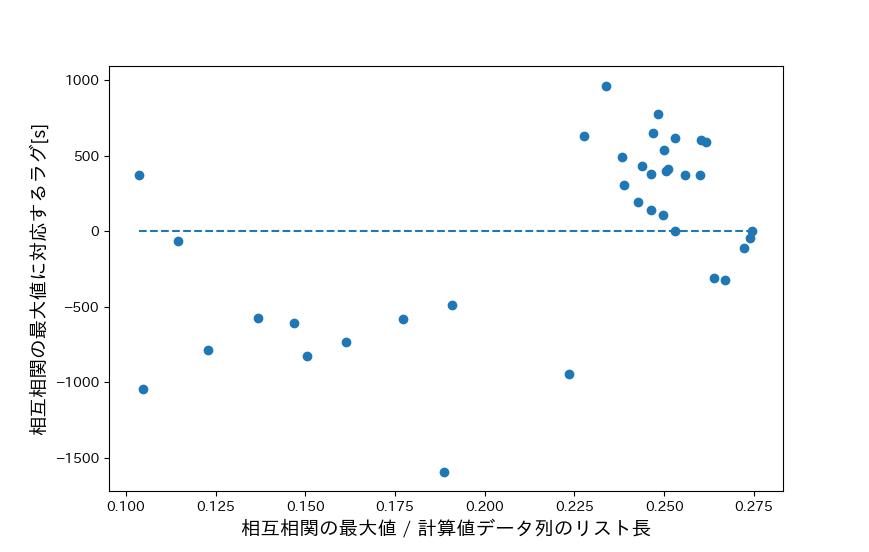
\includegraphics[width=160mm]{1.png}
    \caption{相互相関の最大値を計算値のデータ列のリスト長で割った値と相互相関の最大値に対応するラグをプロットしたもの}
    \label{p1}
  \end{center}
\end{figure}

\section{おわりに}
今回は, 上述の手法によるラグ選定アルゴリズムを実装するにあたり, 相互相関の最大値を計算に使用した計算値データのリスト長で割った値と, その時の相互相関の最大値に対応するラグとの関係について調査した.

その結果, 相互相関の最大値を計算値のデータ列のリスト長で割った値が大きくなるにつれて, その時の相互相関の最大値に対応するラグが0 \si{\second}に近づくことはなかった.

そのため, 相互相関の最大値を計算値のデータ列のリスト長で割った値が, 設定したしきい値を上回るまで再帰的に相互相関の計算に使用する実測データの期間を拡大させることで最適なラグを求める手法には, 事前に実測値と計算値の比を求め, しきい値を下回る比を取る実測値のみになるようフィルタリングするなどといった処理を事前に行う必要があるのではないかという結論に至った.

\begin{thebibliography}{5}
  \bibitem{1}祖父江,"第8回報告書", teams内,参照 July 19, 2022.
\end{thebibliography}

\end{document}